\appendix
\section{Metriche}
  \subsection{Metriche per i processi}
  Metriche di utilità:
    \begin{itemize}
      \item \textbf{Earned value} (EV): valore del lavoro completato fino al momento del calcolo;
      \item \textbf{Planned value} (PV): valore del lavoro come da pianificazione al momento del calcolo;
      \item \textbf{Actual cost} (AC): l'importo speso per il progetto fino al momento del calcolo;
      \item \textbf{Estimate to Completion} (ETC): l'importo previsto che verrà speso per completare la parte restante del progetto al momento del calcolo;
      \item \textbf{Budget at Completion} (BAC): è il budget totale assegnato al progetto.
    \end{itemize}
  Vengono utilizzate le seguenti metriche per valutare l'efficienza e l'efficacia dei processi.
    \subsubsection{MPC1 Schedule Variance (SV)}
    Determina l'anticipo o ritardo nello svolgimento dei processi. È ottenibile attraverso la seguente formula:
      \begin{center}SV = EV - PV.\end{center}
    
    \subsubsection{MPC2 Budget Variance (BV)}
    Determina se si è sotto budget o oltre il budget. È ottenibile attraverso la seguente formula:
      \begin{center}BV = EV - AC.\end{center}

    \subsubsection{MPC3 Estimated at Completion(EAC)}
    Determina il costo previsto del progetto, man mano che il progetto procede. È ottenibile attraverso la seguente formula:
      \begin{center}EAC = AC + ETC.\end{center}
    
    \subsubsection{MPC4 Variance at Completion (VAC)}
    È una proiezione dell'eccedenza o del deficit di bilancio. È ottenibile attraverso la seguente formula:
      \begin{center}VAC = BAC - EAC.\end{center}
  
    \subsubsection{Grafico degli scostamenti}
    \begin{figure}[H]
      \centering
    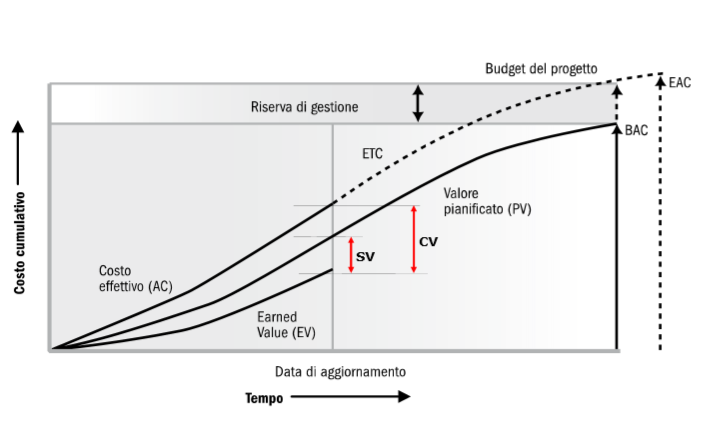
\includegraphics[width=\textwidth,height=\textheight,keepaspectratio]{immagini/graficoPJ.png}
        \caption{Grafico degli scostamenti}
    \end{figure}

  \subsection{Metriche per i prodotti}
  Vengono utilizzate le seguenti metriche per valutare l'efficienza e l'efficacia dei prodotti.
    \subsubsection{MPD1 Indice di Gulpease}
    Determina l'indice di leggibilità del testo. Esso considera il numero di frasi e lettere rispetto al numero di parole. È ottenibile attraverso la seguente formula:
      \begin{displaymath}{IG \: = \: 89 + {300 \: * \: num. \: frasi - 10 \: * \: num. \: lettere \over num. \: parole}}\end{displaymath}
  
    \subsubsection{MPD2 Correttezza ortografica}
    Gli errori ortografici possono essere verificati tramite Spell Right, lo strumento integrato di Visual Studio Code per il controllo ortografico.
    Se presenti, i \textit{verificatori} li correggeranno.
    
    \subsubsection{Metriche per il software}
      \subsubsection{MPS1 Copertura dei requisiti}
      Indica la percentuale di requisiti coperti dall'implementazione. È ottenibile attraverso la seguente formula:
        \begin{displaymath}{C \: = \: (1 \: - \: {N\textsubscript{FM} \over N\textsubscript{FI}}) \: * \: 100}\end{displaymath}
          dove N\textsubscript{FM} è il numero di funzionalità mancanti all'implementazione e N\textsubscript{FI} è il numero di funzionalità individuate nell'attività di analisi.
 
      \subsubsection{MPS2 Tolleranza ai guasti}
      Indica la percentuale di operazioni di testing che si sono concluse in failure. È ottenibile attraverso la seguente formula:
        \begin{displaymath}{F \: = \: {N\textsubscript{FR} \over N\textsubscript{TE}} \: * \: 100}\end{displaymath}
          dove N\textsubscript{FR} è il numero di failure rilevati durante l'attività di testing e N\textsubscript{TE} è il numero di test case eseguiti.
      
      \subsubsection{MPS3 Comprensibilità delle funzionalità offerte}
      Indica la percentuale di operazioni comprese dall'utente senza la consultazione del manuale. È ottenibile attraverso la seguente formula:
        \begin{displaymath}{C \: = \: {N\textsubscript{FC} \over N\textsubscript{FO}} \: * \: 100}\end{displaymath}
          dove N\textsubscript{FC} è il numero di funzionalità comprese in modo immediato dall'utente e N\textsubscript{FO} è il numero di funzionalità totali offerte dal sistema.
      
      \subsubsection{MPS4 Tempo di risposta}
      Indica la differenza di tempo media trascorsa tra l'esecuzione di una funzionalità e la restituzione dell'eventuale risultato finale. È ottenibile attraverso la seguente formula:
        \begin{displaymath}{T\textsubscript{RISP} \: = \: {\sum_{i=1}^n{T\textsubscript{\textit{i}}} \over n}}\end{displaymath}
          dove T\textsubscript{i} è il tempo in secondi trascorso tra la richiesta \textit{i} di una funzionalità e il completamento della stessa con eventuale restituzione di un risultato.
      
      \subsubsection{MPS5 Capacità analisi failure}
      Indica la percentuale di failures incontrate delle quali sono state individuate le cause. È ottenibile attraverso la seguente formula:
        \begin{displaymath}{I \: = \: {N\textsubscript{FI} \over N\textsubscript{FR}} \: * \: 100}\end{displaymath}
          dove N\textsubscript{FI} è il numero di failures delle quali sono state individuate le cause e N\textsubscript{FR} è il numero di failures rilevate.
  
      \subsubsection{MPS6 Impatto delle modifiche}
      Indica la percentuale di modifiche atte a risolvere failures che però hanno introdotto ulteriori failures. È ottenibile attraverso la seguente formula:
        \begin{displaymath}{I \: = \: {N\textsubscript{FRF} \over N\textsubscript{FR}} \: * \: 100}\end{displaymath}
          dove N\textsubscript{FRF} è il numero di failure risolte introducendo nuove failure e N\textsubscript{FR} è il numero di failures risolte.
  

